\chapter{Turbulence Modelling} % Main chapter title
\label{Chapter2}

\section{Viscosity-Based Models}
Violeau et al. \parencite{VIOLEAU2002} were amongst the early pioneers who tried to incorporate a turbulence model in SPH. They came up with two techniques to tackle the problem of turbulence in a Lagrangian framework, which so far had been neglected till then in research, namely, the eddy viscosity model and a generalised Langevin model. For each of their techniques, they considered the following equation of state \ref{eq:violeau-eos}, continuity equation \ref{eq:violeau-continuity} and momentum equation \ref{eq:violeau-mom}, based on the work of \parencite{Monaghan1992}:

\begin{equation}
    P_i = \frac{\rho_0 c_s^2}{\gamma} \Bigg[ \bigg( \frac{\rho_i}{\rho_0} \bigg)^{\gamma} - 1 \Bigg]
    \label{eq:violeau-eos}
\end{equation}
\begin{equation}
    \LagDerivative{\rho_i} = \sum_j m_j \VIJ \cdot \DWIJ
    \label{eq:violeau-continuity}
\end{equation}
\begin{equation}
    \LagDerivative{\vect{v}_i} = \sum_j m_j \bigg( \frac{P_i}{\rho_i^2} + \frac{P_j}{\rho_j^2} + \Pi_{ij} \bigg) \DWIJ + \vect{F}_i
    \label{eq:violeau-mom}
\end{equation}

Where the viscous term is defined as:
\begin{equation}
    \Pi_{ij} = - \frac{16\nu}{\rho_i + \rho_j} \frac{\VIJ \cdot \RIJ}{\RtwoIJ + \MachineEpsilon^2} 
    \label{eq:violeau-diffusion-term}
\end{equation}

\subsection{Eddy Viscosity Model}
\label{sec:eddy-visc-model}

The eddy viscosity model was devised as a first-order closure model, which consisted of a relationship between the Reynolds stress tensor and the mean velocity gradients. Therefore, the momentum equation is similar to the momentum equation, except that the kinematic viscosity is replaced by the eddy viscosity $(\nu_t)$, and the velocities are Reynolds-averaged. In the SPH formalism, the diffusion term occurring is therefore defined as given in \ref{eq:violeau-turbulent-diffusion-term}, with the eddy viscosity defined according to \ref{eq:violeau-eddy-viscosity}.
\begin{equation}
    \Tilde{\Pi}_{ij} = -8 \frac{\nu_{t, i} + \nu_{t, j}}{\rho_i + \rho_j} \frac{\RAProp{\vect{v}}_{ij} \cdot \RIJ }{\RtwoIJ + \MachineEpsilon^2}
    \label{eq:violeau-turbulent-diffusion-term}
\end{equation}
\begin{equation}
    \nu_t = L_m^2 \FrobeniusNorm{S} = L_m^2 \sqrt{\FrobeniusInnerProduct{S}{S}}
    \label{eq:violeau-eddy-viscosity}
\end{equation}

Where $\RAProp{\vect{v}}$ is Reynolds-averaged velocity, and $L_m$ refers to the mixing length scales. The SPH formulation for the mean velocity gradients are given in \ref{eq:violeau-mean-velocity-gradient}.

\begin{equation}
    \nabla \RAProp{\vect{v}}_i = - \frac{1}{\rho_i} \sum_j m_j \RAProp{\vect{v}}_{ij} \otimes \DWIJ
    \label{eq:violeau-mean-velocity-gradient}
\end{equation}

On simulating Poiseuille flow for a high Reynolds number case, the authors could show that the velocity profile showed only a slight discrepancy with theory, with the expected log-law profile near the walls \ref{fig:violeau2002-eddy-viscosity-result}. This indicated that the model is appropriate for turbulent mixing problems or for cases involving spatially-varying viscosity while restricted to shear flows.

\begin{figure}[h]
    \centering
    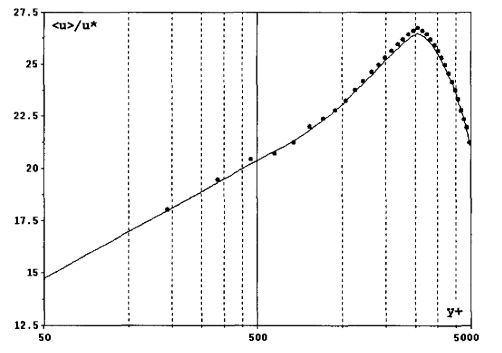
\includegraphics{Figures/research_papers/violeau2002-eddy-viscosity-result.png}
    \caption{Turbulent Poiseuille flow in a pipe $(Re = 64e3)$ modelled using the eddy viscosity model. Computed mean velocity profiles after $(t=1s)$ (solid circles), against theory (solid line). Ref: \parencite{VIOLEAU2002}}
    \label{fig:violeau2002-eddy-viscosity-result}
\end{figure}

\subsection{Generalized Langevin Model}
Violeau et al. also considered a stochastic approach, where the main idea is built on the concept of prescribing particle velocities as a random process, with properties fulfilling the theoretical turbulence hypotheses \parencite{pope1994lagrangi}. Hence, came about the Generalised Langevin model (GLM), where the particle acceleration is defined as:
\begin{equation}
    d\vect{v} = -\frac{1}{\rho} \nabla \RAProp{P} + \tensor{G}(\vect{v} - \RAProp{\vect{v}})dt + \sqrt{C_0 \epsilon dt}\vect{\xi}
    \label{eq:violeau-glm-particle-accel}
\end{equation}

Where $\Vec{\xi}$ is a random vector statistically non-correlated with velocities. The closure for this model was defined by specifying $\tensor{G}$ as:
\begin{equation}
    \tensor{G} = \HalfFrac C_1 \frac{\epsilon}{k}\tensor{I} + C_2 \nabla \RAProp{\vect{v}}
\end{equation}

Where $(k)$ is the turbulent kinetic energy, $(E)$ the dissipation rate, and $(C_i)$ being constants - $(C_1=1.8, C_2=0.6)$.
By modelling turbulence as GLM in SPH, the momentum equation derived was given by:
\begin{equation}
    \LagDerivative{\vect{v}_i} = -\sum_j m_j \bigg( \frac{\RAProp{P}_i}{\rho_i^2} + \frac{\RAProp{P}_j}{\rho_j^2} \bigg) \DWIJ - \HalfFrac C_1 \frac{\epsilon_i}{k_i} \vect{v}'_i + C_2 \nabla \RAProp{\vect{v}}_i \cdot \vect{v}'_i + \sqrt{\frac{C_0 \epsilon_i}{\delta t}} \Vec{\xi}_i
    \label{eq:violeau-mom-glm}
\end{equation}
\begin{equation}
    \RAProp{\vect{v}} = \sum_j \frac{m_j}{\rho_j}\vect{u}_j W_h (\vect{r}_j)
    \label{eq:violeau-ra-vel}
\end{equation}

Where the fluctuations are defined as $\vect{v}' = \vect{v} - \RAProp{\vect{v}}$, and the local values of turbulent kinetic energy and dissipation rate are:
\begin{align}
    \epsilon_i = 2 \nu_{t, i} + 
    \FrobeniusNorm{S_i}^2 \\
    k_i = \frac{\epsilon_i \nu_{t, i}}{C_{\mu}}, C_{\mu} = 0.009
    \label{eq:violeau-k-eps}
\end{align}

It is to be noted that the authors did not estimate the dissipation rate through the proper velocity gradients since the fluctuations of random velocities do not reproduce the small eddies.
The same test case as mentioned in \ref{sec:eddy-visc-model} was considered for the performance of GLM. 
The authors observed large fluctuations. They attributed the discrepancy to the mean operator being redefined as given by \ref{eq:violeau-ra-vel} instead of being a Reynolds average. In fact, by redefining the mean operator in such a fashion, they appeared to have constructed a rudimentary LES filter. 
As observed in \ref{fig:violeau2002-GLM-result}, the fluctuations have an order of magnitude of $k^{1/2}$. However, as claimed by the authors, unlike the eddy viscosity model, the GLM method can be used for different flows instead of being restricted to only shear flows.
\begin{figure}[h]
    \centering
    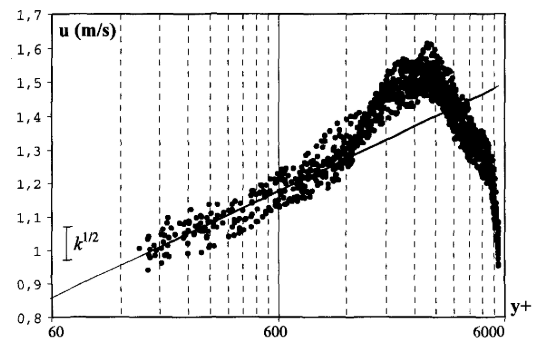
\includegraphics{Figures/research_papers/violeau2002-GLM-result.png}
    \caption{Turbulent Poiseuille flow in a pipe $(Re = 64e3)$ modelled using the generalised Langevin model. Computed mean velocity profiles after $(t=1s)$ (solid circles), against theory (solid line). Ref: \parencite{VIOLEAU2002}}
    \label{fig:violeau2002-GLM-result}
\end{figure}


\section{mSPH}
Adami et al. \parencite{Adami2012} devised a model built on their observation of SPH simulations, wherein the absence of viscosity in typical SPH formulations produced purely noisy particle motion. At finite viscosities, the method would over-predict dissipation. Hence to counter this, they essentially "modified" (hence the name: Modified SPH [mSPH]) the momentum equation and the equation of state to advect the particles in order to homogenise the particle distribution, in turn stabilising the numerical scheme. They were also able to reduce the artificial dissipation in transitional flows.

The authors considered summation density (\ref{eq:Adami2012-summation-density}), which is a function of the volume of the respective SPH particle as given by \ref{eq:Adami2012-vol}, as opposed to evolving density through the continuity equation \parencite{hu2006multi}. The modified equation of state as given by \ref{eq:Adami2012-eos}, is equivalent to the classical SPH equation-of-state with $\gamma=1$.
\begin{equation}
    \Vol_i = \frac{1}{\sum_j \WIJ}
    \label{eq:Adami2012-vol}
\end{equation}
\begin{equation}
    \rho_i = \frac{m_i}{\Vol_i} = m_i\sum_j \WIJ
    \label{eq:Adami2012-summation-density}
\end{equation}
\begin{equation}
    P_i = c_s^2 (\rho_i - \rho_0)
    \label{eq:Adami2012-eos}
\end{equation}

The momentum equation, which provides the acceleration of the particle, is a function of just the gradient and viscous shear forces as given by \ref{eq:Adami2012-mom-governing}. The corresponding SPH formulation was derived as given by \ref{eq:Adami2012-mom-sph}, which built on the earlier work of Hu and Adams \parencite{hu2007incompressible}.
\begin{equation}
    \LagDerivative{\vect{v}} = -\frac{1}{\rho}\nabla P + \nu \Delta( \vect{v} ) + \vect{F}
    \label{eq:Adami2012-mom-governing}
\end{equation}
\begin{equation}
    \LagDerivative{\vect{v}_i} = -\frac{1}{m_i} \sum_j (\Vol^2_i + \Vol^2_j) \frac{P_i \rho_j + P_j \rho_i}{\rho_i + \rho_i} \DWIJ - \frac{\eta}{m_i} \sum_j (\Vol^2_i + \Vol^2_j) \frac{\VIJ}{\RtwoIJ[]}\DWIJ + \vect{F}_i
    \label{eq:Adami2012-mom-sph}
\end{equation}

This scheme takes advantage of the regularisation of the
particle motion stemming from the additional background pressure $(P_0 = \rho_0 c_s^2)$. The additional force exerted by the background pressure counteracts non-homogeneous particle distributions, therein reducing numerical dissipation.

The authors estimated the energy spectra of the flow simulations in order to analyse the results of their test cases, using first and second-order moving-least-squares (MLS) method \parencite{gossler2001moving} and its subsequent Fourier transform \parencite{frigo2005design}.
Their first test case, the $2D$ variant of the Taylor-Green Vortex (TGV) problem, involved $8\times 8$ counter-rotating vortices, requiring $64^2$ particles. They considered the viscosity to be zero.
As seen in the time evolution of the 
\begin{figure}[h]
    \centering
    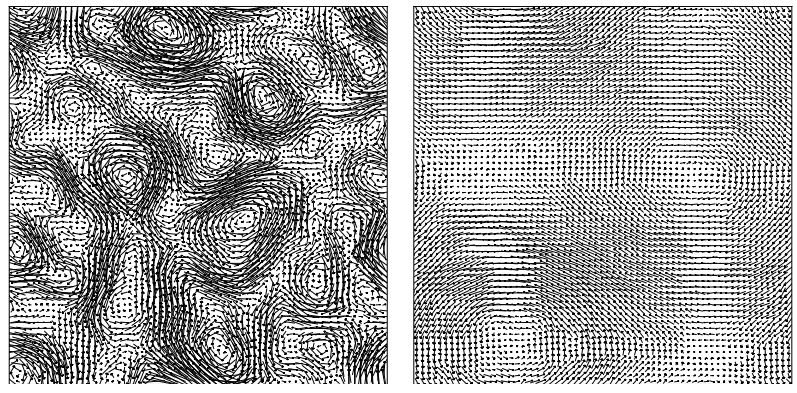
\includegraphics[scale=0.7]{Figures/research_papers/adami2012-evolution-vel-field-tgv.png}
    \caption{Velocity vector plot at $t=2$ (left) and $t=30$ (right). $Re = \infty$. Ref: \parencite{Adami2012} }
    \label{fig:adami2012-evolution-vel-field-tgv}
\end{figure}

The time evolution of the velocity field is given in \ref{fig:adami2012-evolution-vel-field-tgv}, where it can be observed that the $2D$ turbulence is characterised by merging and pairing of small vortices. The energy spectra given in \ref{fig:adami2012-energy-spectra-tgv} show that at low wave numbers, both interpolation schemes give the same results, but at high wave numbers, the results differ. The energy spectrum of the standard SPH has a linear slope of magnitude $m = 1$ in a log-log scale equivalent to a purely noisy velocity field. Theoretically, however, $2D$ turbulence has an energy cascade with a slope of $m = -3$ in the inertial range, which is reasonably predicted using mSPH.
\begin{figure}[h]
    \centering
    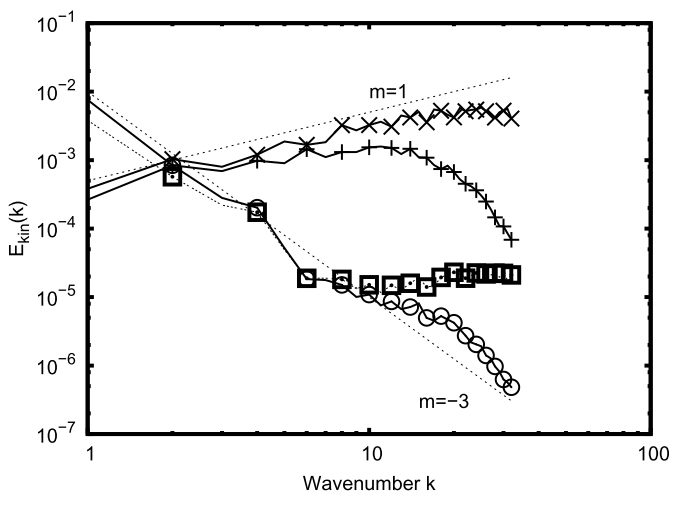
\includegraphics[scale=0.55]{Figures/research_papers/adami2012-energy-spectra-tgv.png}
    \caption{Comparison of energy spectra $t=10$. $+$ and $\times$ denote standard SPH results with quintic spline and MLS interpolation; $\circ$ and $\square$ denote mSPH results with quintic spline and MLS interpolation. Ref: \parencite{Adami2012} }
    \label{fig:adami2012-energy-spectra-tgv}
\end{figure}

The second test case employed by the authors was that of the $3D$ TGV problem requiring $64^3$ particles for a wide range of Reynolds numbers. The dissipation rate of the flow simulations are shown in \ref{fig:adami2012-dissipation-re400} and \ref{fig:adami2012-dissipation-re3000}. It can be observed that the standard SPH is unable to simulate transitional flows due to excessive dissipation. In contrast, mSPH can reproduce the dissipation rate reasonably well. This implies that the corrected particle transport velocity is an analogous eddy-viscosity model on scales below the numerical resolution.
\begin{figure}[h]
    \centering
    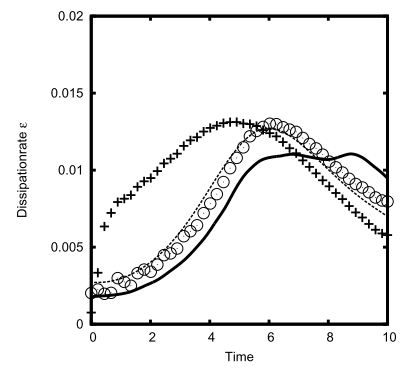
\includegraphics[scale=0.7]{Figures/research_papers/adami2012-dissipation-re400.png}
    \caption{Dissipation rate at $Re = 400$ using DNS (solid line), Smagorinsky model (dashed line), standard SPH ($+$) and mSPH ($\circ$). Ref: \parencite{Adami2012}}
    \label{fig:adami2012-dissipation-re400}
\end{figure}
\begin{figure}[h]
    \centering
    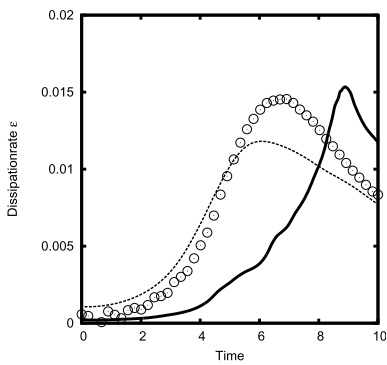
\includegraphics[scale=0.7]{Figures/research_papers/adami2012-dissipation-re3000.png}
    \caption{Dissipation rate at $Re = 3000$ using DNS (solid line), Smagorinsky model (dashed line) and mSPH ($\circ$). Ref: \parencite{Adami2012}}
    \label{fig:adami2012-dissipation-re3000}
\end{figure}

\section{Large Eddy Simulation-based Models}
\subsection{Implicit Pressure Poisson-based Models}
Gotoh et. al \parencite{Gotoh2004} were amongst the first to integrate Large Eddy Simulation techniques with SPH method. They derived this LES-SPH model, based on incompressible flow, so as to tackle the problem of reflection and transmission characteristics of regular waves by a partially immersed curtain-type breakwater. In order to compare the dissipation efficiencies, they considered the non-overtopping and overtopping cases of the problem.

The governing equations of the system was described as given by the continuity equation in \ref{eq:Gotoh2004-continuity-governing} and momentum equation in \ref{eq:Adami2012-mom-governing}.
\begin{equation}
    \frac{1}{\rho} \LagDerivative{\rho} + \nabla \cdot \vect{v} = 0
    \label{eq:Gotoh2004-continuity-governing}
\end{equation}

The LES mass and momentum conservation equations for the flow was derived by filtering the respective equations using a spatial filter $\overline{(...)}$ to obtain their filtered counter-parts as given by \ref{eq:Gotoh2004-continuity-filtered} and \ref{eq:Gotoh2004-mom-filtered} respectively.
\begin{equation}
    \frac{1}{\rho} \LagDerivative{\rho} + \nabla \cdot \vect{\overline{v}} = 0
    \label{eq:Gotoh2004-continuity-filtered}
\end{equation}
\begin{equation}
    \LagDerivative{\vect{\overline{v}}} = -\frac{1}{\rho}\nabla \overline{P} + \nu \Delta ( \vect{\overline{v}} ) + \frac{1}{\rho}\nabla\cdot\tensor{\tau} + \vect{F}
    \label{eq:Gotoh2004-mom-filtered}
\end{equation}
\begin{equation}
    \frac{1}{\rho} \tensor{\tau} = \vect{\overline{v}} \otimes \vect{\overline{v}} - \overline{\vect{v} \otimes \vect{v}}
    \label{eq:Gotoh2004-stress-tensor}
\end{equation}

The stress tensor defined in \ref{eq:Gotoh2004-stress-tensor} is closed using the Boussinesq's Hypothesis as defined in \ref{eq:Gotoh2004-boussinesq}.
\begin{equation}
    \frac{1}{\rho} \tensor{\tau} = 2\nu_t \tensor{S} - \frac{2}{3}k\tensor{I}
    \label{eq:Gotoh2004-boussinesq}
\end{equation}

The turbulent eddy viscosity is estimated using a modified Smagorinsky model as given in \ref{eq:Gotoh2004-eddy-visc}. This allows wall effects to be incorporated in the model, which was required by the authors in order to tackle the problem they were working on.
\begin{equation}
    \nu_t = \min(C_s \Delta x, \kappa d_{wall})^2 \sqrt{2 \FrobeniusInnerProduct{S}{S}}
    \label{eq:Gotoh2004-eddy-visc}
\end{equation}
\begin{equation}
    C_s=0.1, \kappa=0.4
\end{equation}

Where, $(C_s)$ is the Smagorinsky constant, $(\kappa)$ is the von Karman constant and $d_{wall}$ is the normal distance of particle to the closest wall.
The first term in \ref{eq:Gotoh2004-eddy-visc} dominates the flow far away from the solid wall, thereby recovering the standard Smagorinsky model. However, for flow close to the wall, the second term dominates and hence the eddy viscosity is a function of the particle distance to the wall. This overcomes the disadvantage of the standard Smagorinsky being over-dissipative inside the laminar layer.

In order to system of equations, and evolve them in time, the authors employed the Predictive-Corrective time integrator, similar to the two-step projection method of Chorin \parencite{chorin1968numerical}. The prediction stage is outlined by \ref{eq:Gotoh2004-predict-start} - \ref{eq:Gotoh2004-predict-end}. 
\begin{equation}
    \Delta \vect{v}_* = \bigg( \nu \Delta ( \vect{\overline{v}} ) + \frac{1}{\rho}\nabla\cdot\tensor{\tau} + \vect{F} \bigg) \Delta t
    \label{eq:Gotoh2004-predict-start}
\end{equation}
\begin{equation}
    \vect{v}_* = \vect{v}_t + \Delta \vect{v}_*
\end{equation}
\begin{equation}
    \vect{r}_* = \vect{r}_t + \vect{v}_* \Delta t
    \label{eq:Gotoh2004-predict-end}
\end{equation}

The correction stage is outlined by \ref{eq:Gotoh2004-correct-start} - \ref{eq:Gotoh2004-correct-end}. $(\overline{P})$ which is required to update the $(\vect{v}_{t+1})$ term is calculated implicitly from \ref{eq:Gotoh2004-correct-pressure-implicit}, which is based on the filtered continuity equation given by \ref{eq:Gotoh2004-continuity-filtered} and assuming incompressibility $\LagDerivative{\rho}=0$.
\begin{equation}
    \Delta \vect{v}_{**} = -\frac{1}{\rho} \nabla \overline{P}_{t+1} \Delta t
    \label{eq:Gotoh2004-correct-start}
\end{equation}
\begin{equation}
    \nabla \cdot \bigg( \frac{1}{\rho_*} \nabla \overline{P}_{t+1} \bigg) = \frac{\rho_0 - \rho_*}{\rho_0 \Delta t^2}
    \label{eq:Gotoh2004-correct-pressure-implicit}
\end{equation}
\begin{equation}
    \vect{v}_{t+1} = \vect{v}_* + \Delta \vect{v}
\end{equation}
\begin{equation}
    \vect{r}_{t+1} = \vect{r}_t + (\vect{v}_t + \vect{v}_{t+1})\frac{\Delta t}{2}
    \label{eq:Gotoh2004-correct-end}
\end{equation}

In order to solve the system of equations given by \ref{eq:Gotoh2004-predict-start} - \ref{eq:Gotoh2004-correct-end} in an SPH setting, the authors presented the following SPH formulation for the flow property. \textit{Note:} The over-line $\overline{(...)}$ convention used to denote filtered flow properties will be dropped in this sub-section, unless stated otherwise.

The fluid density is given using a simple summation density \ref{eq:Gotoh2004-summation-density}.
\begin{equation}
    \rho_i = \sum_j m_j\WIJ
    \label{eq:Gotoh2004-summation-density}
\end{equation}

The pressure gradient term is defined in \ref{eq:Gotoh2004-grad-p-sph} in a symmetric form.
\begin{equation}
    \bigg( \frac{1}{\rho} \nabla P \bigg)_i = \sum_j m_j \bigg( \frac{P_i}{\rho_i^2} + \frac{P_j}{\rho_j^2} \bigg) \DWIJ
    \label{eq:Gotoh2004-grad-p-sph}
\end{equation}

The divergence of $\vect{v}$ is also defined symmetrically as given by \ref{eq:Gotoh2004-div-u-sph}.
\begin{equation}
    \nabla \cdot \vect{v}_i = \rho_i \sum_j m_j \bigg(\frac{\vect{v}_i}{\rho^2_i} + \frac{\vect{v}_j}{\rho^2_j} \bigg) \cdot \DWIJ
    \label{eq:Gotoh2004-div-u-sph}
\end{equation}

The pressure Laplacian, defined in \ref{eq:Gotoh2004-p-laplacian-sph}, is formulated as a hybrid of a standard SPH first derivative with a finite difference approximation for the first derivative, so as to aid particle pressure stability \parencite{cummins1999sph}.
\begin{equation}
    \nabla \cdot \bigg( \frac{1}{\rho} \nabla P \bigg)_i = \sum_j m_j \frac{8}{(\rho_i + \rho_j)^2} \frac{P_{ij} \RIJ \cdot \DWIJ }{\RtwoIJ}
    \label{eq:Gotoh2004-p-laplacian-sph}
\end{equation}

The divergence of the stress tensor is defined in \ref{eq:Gotoh2004-div-tau-sph}.
\begin{equation}
    \bigg( \frac{1}{\rho} \nabla \cdot \tensor{\tau} \bigg)_i = \sum_j m_j \Bigg( \frac{1}{\rho_i^2}\tensor{\tau_i} + \frac{1}{\rho_j^2}\tensor{\tau_j} \Bigg) \cdot \DWIJ
    \label{eq:Gotoh2004-div-tau-sph}
\end{equation}

Finally the laminar stress term, consisting of the velocity Laplacian term, is defined as given by \ref{eq:Gotoh2004-vel-laplacian-sph}.
\begin{equation}
    \big(\nu \Delta(\vect{v}) \big)_i = \sum_j m_j \frac{4(\eta_i + \eta_j)}{(\rho_i + \rho_j)^2}\frac{\VIJ \RIJ \cdot \DWIJ}{\RtwoIJ}
    \label{eq:Gotoh2004-vel-laplacian-sph}
\end{equation}

The authors used this SPH-LES model to investigate the wave interaction with partially immersed breakwater, and compared the results with experimentally obtained values of a similar setup. Their computational domain was $2D$ populated by $\approx 12e3$ particles.

\begin{figure}[h]
    \centering
    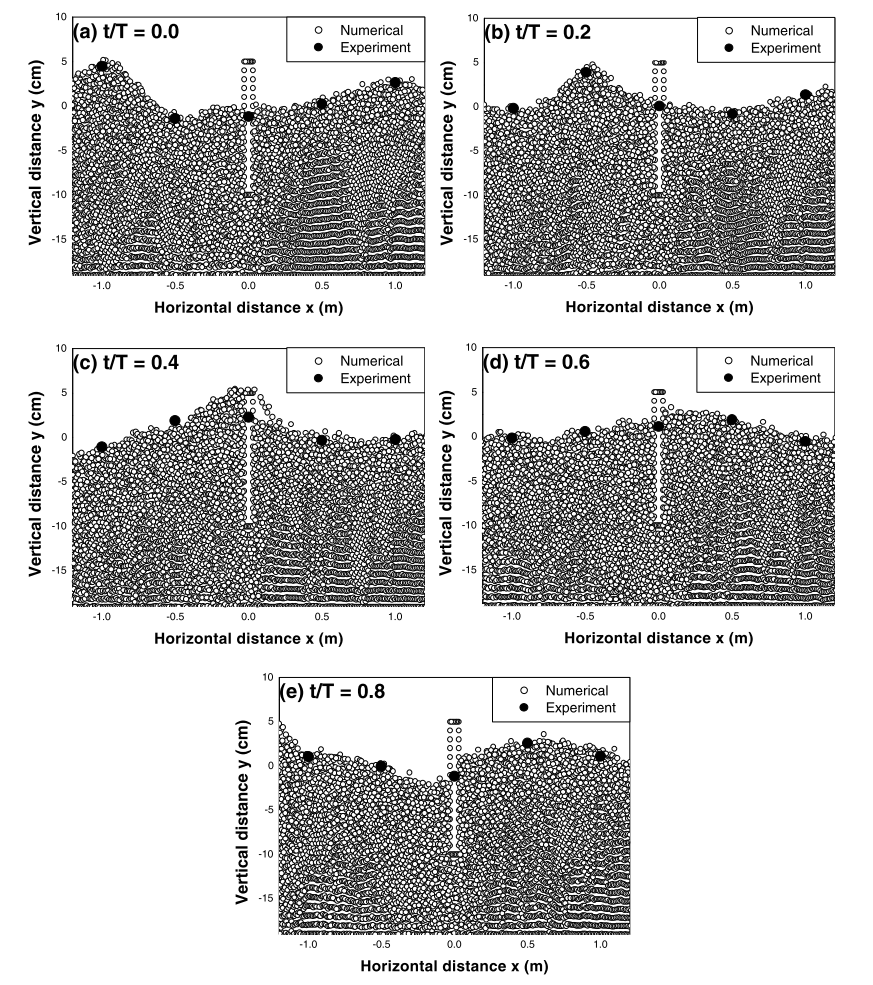
\includegraphics[scale=0.8]{Figures/research_papers/gotoh2004-wave-profile-result.png}
    \caption{Time sequences of computational and experimental wave profiles near curtain wall (overtopping). Ref: \parencite{Gotoh2004}}
    \label{fig:gotoh2004-wave-profile-result}
\end{figure}

As observed in the comparative plots given in \ref{fig:gotoh2004-wave-profile-result}, the model proves to be accurate in tracking free-surfaces of large deformation without numerical diffusion. The authors also observed the capability of the model in simulating turbulence and eddy vortices realistically near the curtain wall. However, the authors also conclude that a more refined turbulence model will be required for further accuracy in predicting flow involving wave interactions.

Building on the work mentioned above, Shao and Gotoh \parencite{Shao2005}, performed a comparative study of SPH and Moving Particle Semi-Implicit (MPS) method coupled with a LES model. They also validated these models against experimental data.

The filtered conservation equations which the authors considered were the same as given by \ref{eq:Gotoh2004-continuity-filtered} - \ref{eq:Gotoh2004-boussinesq}. However, they incorporated the standard Smagorinsky model \parencite{smagorinsky1963general} given by \ref{eq:Shao2005-eddy-visc} as opposed to the modified model \ref{eq:Gotoh2004-eddy-visc}.
\begin{equation}
    \nu_t = (C_s \Delta x)^2
    \label{eq:Shao2005-eddy-visc}
\end{equation}

The authors consider the same predictive-corrective scheme to evolve their system as detailed in \ref{eq:Gotoh2004-predict-start} - \ref{eq:Gotoh2004-correct-end}.
Similarly, they follow the same SPH formulation outlined in \ref{eq:Gotoh2004-summation-density} - \ref{eq:Gotoh2004-vel-laplacian-sph}. They do however, slightly modify the pressure and velocity Laplacian terms as given in \ref{eq:Shao2005-P-laplacian-sph} and \ref{eq:Shao2005-vel-laplacian-sph} respectively.
\begin{equation}
    (\nabla^2 P)_i = \sum_j m_j \frac{4}{\rho_i + \rho_j} \frac{P_{ij} \RIJ \cdot \DWIJ }{\RtwoIJ}
    \label{eq:Shao2005-P-laplacian-sph}
\end{equation}
\begin{equation}
    \big(\nu \Delta(\vect{v}) \big)_i = \sum_j m_j \frac{2(\nu_i + \nu_j)}{\rho_i + \rho_j}\frac{\VIJ \RIJ \cdot \DWIJ}{\RtwoIJ}
    \label{eq:Shao2005-vel-laplacian-sph}
\end{equation}

The authors validated this SPH-LES Model using experimental data from the experimental data corresponding to a solitary wave breaking on the beach \parencite{Synolakis1986}. Their computational domain was $2D$ and consisted of $\approx 18e3$ particles. 
From the computed wave profiles shown in \ref{fig:shao2005-wave-profile-result}, it can be visually observed that there is reasonable agreement between the experimental and computation data. This again verifies the accuracy of the model in tracking free surfaces with less or no numerical diffusion.
Furthermore, by performing a convergence study of the SPH-LES model using the dam-break problem, the authors were able to show that the spatial and temporal accuracy of the scheme is $O(\Delta t + \Delta x^(1.25)$.

\begin{figure}[h]
    \centering
    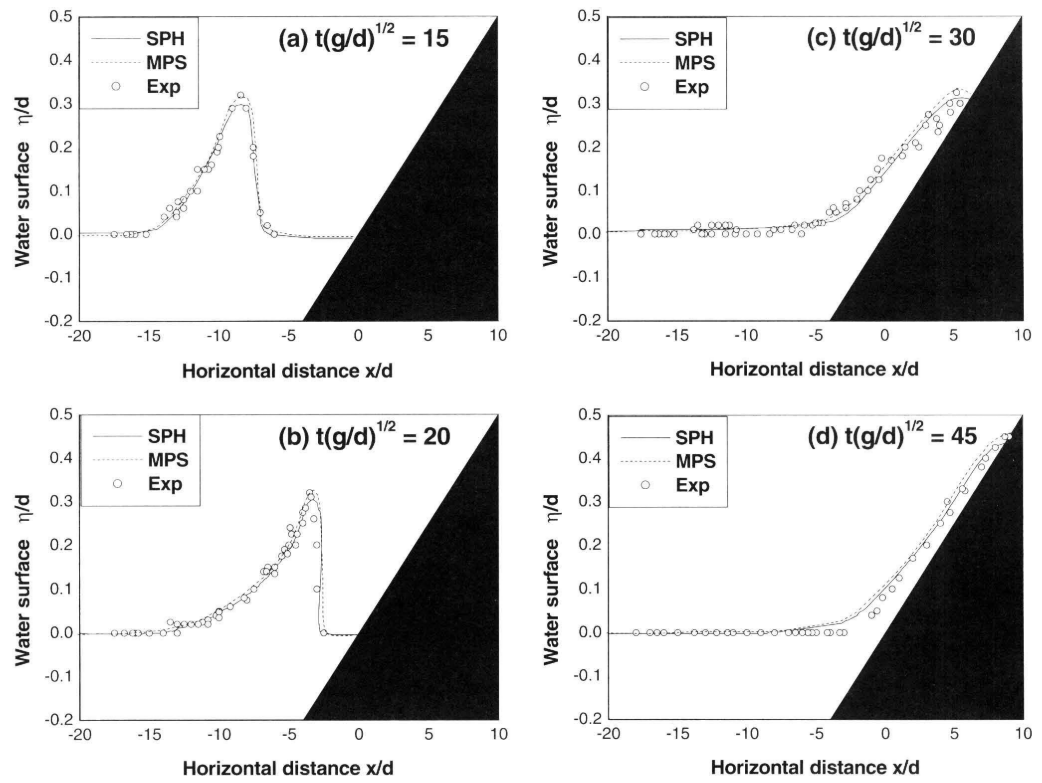
\includegraphics[scale=0.6]{Figures/research_papers/shao2005-wave-profile-result.png}
    \caption{Experimental and computational wave profiles by SPH and MPS model. Ref: \parencite{Shao2005}}
    \label{fig:shao2005-wave-profile-result}
\end{figure}


\subsection{Explicit Pressure Equation of State-based Solvers}
Weakly compressible solvers